\documentclass[conference]{IEEEtran}
\IEEEoverridecommandlockouts
% The preceding line is only needed to identify funding in the first footnote. If that is unneeded, please comment it out.
\usepackage{cite}
\usepackage{amsmath,amssymb,amsfonts}
\usepackage{algorithmic}
\usepackage{graphicx}
\usepackage{textcomp}
\usepackage{xcolor}
\usepackage{hyperref}
\usepackage{listings}
\usepackage{float}

\def\BibTeX{{\rm B\kern-.05em{\sc i\kern-.025em b}\kern-.08em
    T\kern-.1667em\lower.7ex\hbox{E}\kern-.125emX}}
    
\begin{document}

\title{App-controlled LEGO 3-DoF robotic arm\\
{\footnotesize Mobile Computing | winter term 2018/2019}
}

\author{
\IEEEauthorblockN{Christoph Ulrich}
\IEEEauthorblockA{%\textit{dept. name of organization (of Aff.)} \\
\textit{HTWG Konstanz}\\
Constance, Germany\\
christoph.ulrich@htwg-konstanz.de}
\and
\IEEEauthorblockN{Benjamin Schaefer}
\IEEEauthorblockA{%\textit{dept. name of organization (of Aff.)} \\
\textit{HTWG Konstanz}\\
Constance, Germany\\
benjamin.schaefer@htwg-konstanz.de}
}

\maketitle

\begin{abstract}
Die folgende Ausarbeitung beschreibt die Berechnung einer einfachen Wellenausbreitungsfunktion mithilfe des CUDA-Frameworks und die Darstellung der berechneten Daten mittels der Grafikbibliothek OpenGL. Ausgangssituation ist dabei eine stillliegende Wasseroberfl\"ache. Simuliert wird die kreisf\"ormige Ausbreitung einer Welle, die etwa von einem ins Wasser geworfenen Stein verursacht worden sein k\"onnte. Die nach Evaluation ausgew\"ahlte Funktion zur Berechnung der Welle wurde zuerst zu Testzwecken auf der CPU implementiert und anschlie{\ss}end in einen CUDA-Kernel \"uberf\"uhrt. Danach wird ein weiterer Kernel konstruiert, mit dem die Oberfl\"ache der errechneten Welle in Dreiecke aufgeteilt und dann mittels OpenGL gerendert wird. Anschlie{\ss}end werden die implementierten Kernel und unterschiedlichen Vorgehensweisen auf ihre Laufzeiten untersucht und verglichen. Zum Schluss erfolgt eine kritische Betrachtung des Projektes in Form von Optimierungsvorschl\"agen und eines Fazits.
\end{abstract}

%\begin{IEEEkeywords}
%component, formatting, style, styling, insert
%\end{IEEEkeywords}\

\section{Planung und Ziele}
Die Vorabplanung des Projektes sah die Simulation einer Wellenausbreitung (z.B. im Medium Wasser) ausgehend von einem Ausbreitungszentrum vor. Die Berechnungen sollten auf einem Grafikprozessor (im Folgenden kurz: GPU) mittels CUDA erfolgen und ein grauwertbild\"ahnliches Format liefern, wobei die einzelnen Pixelwerte die H\"ohe der Welle an der jeweiligen Stelle repr\"asentieren sollten. Im Anschluss daran sollte aus den berechneten Daten ein Mesh generiert und dieses mittels OpenGL \textit{gerendert} werden. Zus\"atzlich zu diesen Grundzielen wurden folgende optionale Ziele (Umsetzung nur bei vertretbarem Aufwand sowie vertretbarer Komplexit\"at) vereinbart:

\begin{itemize}
\item Setzen des Ausbreitungszentrums per Mausklick
\item Darstellung mehrerer Wellen mit unterschiedlichen Ausbreitungszentren und Wellen\"uberlagerung
\item Rendern mit Textur
\end{itemize}

\section{Vorarbeiten}

\subsection{Finden einer geeigneten Wellenfunktion}
Zu Beginn galt es, eine Wellenfunktion zu finden, die den gew\"unschten Anforderungen entspricht, d.h. eine kreisf\"ormige, mit der Zeit abschw\"achende und dreidimensionale Ausbreitung beschreibt. Am Ende der Recherche standen die nachfolgenden drei Ausbreitungsfunktionen zur Auswahl:

\begin{equation}\label{eq:wave}
\eta(r, \theta, t) = \frac{\sqrt[]{gt}}{r^{\frac{5}{2}}} \cdot (\cos(\frac{gt^{2}}{4r}) - \sin(\frac{gt^{2}}{4r}))
\end{equation}
$r$ und $\theta$ beschreiben hier die Polarkoordinaten der Welle.

\begin{figure}[H]
\centerline{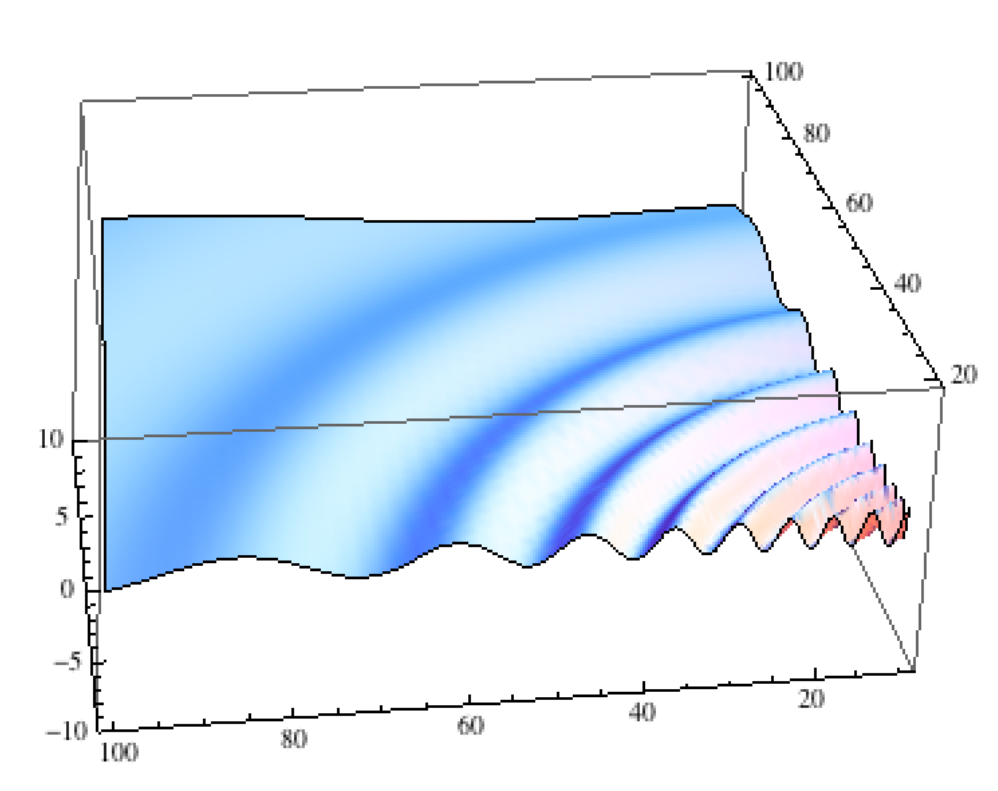
\includegraphics[scale=0.25]{img/wave1.png}}
\label{fig:wave}
\caption{3D-Python-Plot zu Funktion \eqref{eq:wave}}
\end{figure}

\begin{equation}\label{eq:drop}
-(\frac{1+\cos(12*\sqrt[•]{x^{2} + y^{2}})}{\frac{1}{2} \cdot ({x^{2} + y^{2}) + 2}})
\end{equation}
$x$ und $y$ beschreiben hier die kartesischen Koordinaten der Welle.

\begin{figure}[H]
\centerline{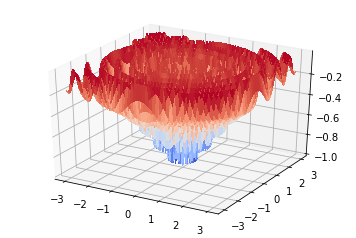
\includegraphics[scale=0.75]{img/drop_wave.png}}
\label{fig:drop_wave}
\caption{3D-Python-Plot zu Funktion \eqref{eq:drop}}
\end{figure}

\begin{equation}\label{eq:ripples}
\frac{\cos(\frac{1}{2} \cdot \sqrt[]{x^{2} + y^{2}} - 6t)}{\frac{1}{2} \cdot (x^{2} + y^{2}) + 1 + 2t}
\end{equation}
$x$ und $y$ beschreiben hier die kartesischen Koordinaten der Welle.

\begin{figure}[H]
\centerline{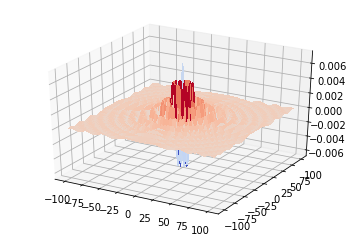
\includegraphics[scale=0.75]{img/ripples.png}}
\label{fig:ripples}
\caption{3D-Python-Plot zu Funktion \eqref{eq:ripples}}
\end{figure}

Funktion \eqref{eq:drop}, die sog. \textit{drop-wave}-Funktion, ber\"ucksichtigt keine zeitliche Entwicklung, sondern berechnet die Wellenausbreitung lediglich zu einem schon fortgeschrittenen Zeitpunkt. Eine M\"oglichkeit h\"atte in der Anpassung der Funktion und dem Einbau eines zeitlichen Parameters bestanden. Aufgrund weiterer zur Verf\"ugung stehender Alternativen wurde jedoch von diesem Vorgehen abgesehen und die Entscheidung fiel zugunsten von Funktion \eqref{eq:ripples}. Neben des relativ einfachen Aufbaus hat diese Ausbreitung den Vorteil eines deutlich sichtbaren Zentrums, was die reale Situation nach Eintauchen eines Objektes in eine Wassermasse hervorhebt. 

\subsection{Konzeptentwurf}
Um von der reinen Formel zur schlussendlichen Visualisierung zu gelangen, wird die Vorgehensweise bei der Datenberechnung in zwei essentielle Schritte eingeteilt, die jeweils geeignete Datenstrukturen ben\"otigen. \\

\subsubsection{H\"ohenfeld}
Die Ergebnisse der Berechnungen mit Funktion \ref{eq:ripples} repr\"asentieren die H\"ohe der Welle an der Position [x,y] zum Zeitschritt $t$, die in einem sog. H\"ohenfeld (engl.: \textit{height field}) hinterlegt werden. Dieses Feld - \"ahnlich einem Grauwertbild - kann entweder als eindimensionale Liste oder als 2D-Grid gespeichert werden. Im ersten Fall wird auf den Wert an der Position [x,y] mit der Index-Umrechnung $y*size_y + x$ (typisches 2D-zu-1D-Mapping) zugegriffen. Das H\"ohenfeld muss zu jedem Zeitschritt $t$ neu berechnet werden.
\\

\subsubsection{Dreiecke}\label{sec:triangles}
Mit den Daten aus dem H\"ohenfeld sind zwar theoretisch alle Informationen zur Wellenstruktur vorhanden. Um die Welle jedoch sp\"ater mit \textit{OpenGL} darstellen zu k\"onnen, m\"ussen die errechneten Punkte aus dem H\"ohenfeld in Dreiecke transformiert werden. 

\begin{figure}[H]
\centerline{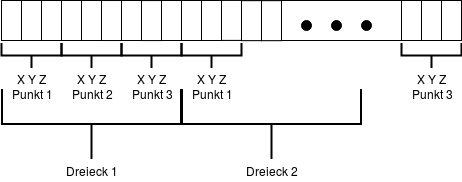
\includegraphics[scale=0.55]{img/triangle.png}}
\label{fig:triangle}
\caption{Datenstruktur der Dreiecke}
\end{figure}

Die Dreieckskoordinaten werden nacheinander in einem Float-Array abgelegt, wobei ein Dreieckspunkt aus drei Werten (x ,y, z) besteht und daraus folgend ein gesamtes Dreieck aus neun Array-Eintr\"agen besteht (siehe Abbildung \ref{fig:triangle})

\section{Implementierung auf der CPU}

Vor Umsetzung auf der GPU wurde die Berechnung der Wellenausbreitung mit klassisch sequentiellem Code auf der CPU implementiert. Damit war es auch m\"oglich, im Voraus die allgemeine Funktionalit\"at und die Korrektheit der Daten zu verifizieren. Dabei wurde mit zwei verschachtelten \textit{for}-Schleifen \"uber die gew\"unschte Anzahl von y- und x-Koordinaten iteriert und die H\"ohe der Welle an der jeweiligen Stelle berechnet. Um eine feinere Aufl\"osung zu erreichen, wurde ein Skalierungsfaktor mit den Koordinaten verrechnet:

\begin{lstlisting}[language=c, caption=Berechnung des H\"ohenfeldes auf der CPU - Pseudo-Code, captionpos=b]
for (y=0; y<size_y; ++y) {
	for (x=0; x<size_x; ++x) {
		float fx=x*scale_x-trans;
		float fy=y*scale_y-trans;
		height_field[y,x] = ...;
\end{lstlisting}

Mit dem resultierenden H\"ohenfeld k\"onnen nun die zur Darstellung notwendigen Dreiecke errechnet werden.

\begin{figure}[H]
\centerline{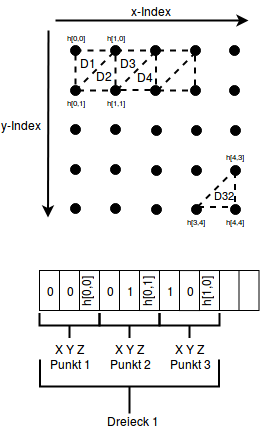
\includegraphics[scale=0.75]{img/triangle_coords_calculation.png}}
\label{fig:triangle_coords_calculation}
\caption{Berechnung der Dreieckskoordinaten}
\end{figure}

Die Dreiecke werden nach dem in Abbildung \ref{fig:triangle_coords_calculation} skizzierten Schema in ein eindimensionales Float-Array $T$ geschrieben. $x$, $y$ und $h[x,y]$ sind die Koordinaten eines zum jeweiligen Dreieck $D_x$ geh\"origen Punktes. Die Anzahl $n_D$ der durch ein H\"ohenfeld $h$ beschriebenen Dreiecke errechnet sich durch

\begin{equation}
n_D = (size_{h_x} - 1) \cdot (size_{y_x} - 1) \cdot 2
\end{equation}

Demnach bel\"auft sich die Gr\"o{\ss}e des Arrays zur Speicherung der Dreieckskoordinaten $T$ auf

\begin{equation}
size_T = n_D \cdot 3 \cdot 3
\end{equation}

F\"ur das in Abbildung \ref{fig:triangle_coords_calculation} gezeigte Beispiel gilt dann:\\ $n_D = (5-1) * (5-1) * 2 = 32$ sowie $size_T = 32 * 9 = 288$
\\
Die CPU-Code-Struktur zur Berechnung der Dreieckskoordinaten gleicht der zur Berechnung des H\"ohenfeldes:

\begin{lstlisting}[language=c, caption=Berechnung der Dreieckskoordinaten auf der CPU - Pseudo-Code, captionpos=b]
for (int y=0; y<(size_y-1); ++y) {
	for (int x=0; x<(size_x-1); ++x) {
\end{lstlisting}

\section{Implementierung auf der GPU}
Im Folgenden ist die Analyse des CPU-Codes hinsichtlich Parallelisierbarkeit und die anschlie{\ss}ende Portierung in parallel ausf\"uhrbaren Code durch Konstruktion geeigneter CUDA-Kernel und Verwendung von Parallelisierungs- und Operation-Pattern beschrieben. 

\subsection{Analyse des CPU-Codes}\label{sec:anal}
Bei Untersuchung der relevanten Anteile des CPU-Codes l\"asst sich feststellen, dass innerhalb der zu parallelisierenden Aufgaben (H\"ohenfeld- und Dreiecksberechnung) keine Abh\"angigkeiten bestehen.
Die Dreiecksberechnung ben\"otigt jedoch als Input das Ergebnis einer abgeschlossenen H\"ohenfeldberechnung, d.h. diese Aufgaben werden sequentiell nacheinander ausgef\"uhrt.
Da, wie in Listing 1. und Listing 2. zu sehen, \"uber for-Schleifen diesselbe Rechenoperationen auf unterschiedliche Daten () angewendet werden, sind die einzelnen Jobs jeweils Daten-parallel und damit hervorragend geeignet f\"ur die Berechnung auf den \textit{SIMD}-Cores der GPU.
Im Hinblick auf die Granularit\"at macht es deswegen Sinn, die Aufgaben jeweils in sehr kleine Teilaufgaben aufzuteilen, d.h. wenige Instruktionen pro Thread und dabei viele Threads zu verplanen.

\subsection{Portierung nach CUDA}\label{sec:port}
Nach erfolgter Analyse l\"asst sich die Strategie zur Parallelisierung nun ...
Aufgrund der Feingranularit\"at der Jobs ist das Ziel, f\"ur die Kernel die maximale Anzahl an Threads auszunutzen. Die beiden bei der  Entwicklung eingesetzten Grafikkarten \textit{GeForce GTX 940M} und \textit{GeForce GTX 960M} sind hardwaretechnisch limitiert auf eine maximale Anzahl von 1024 Threads pro Block. Aufgrund einfacher Indizierung der 2D-Daten werden quadratische 2D-Blocks mit 32x32 Threads eingesetzt. Anhand der Gr\"o{\ss}e der Wasseroberfl\"ache wird die Dimensionierung des 2D-Block-Grids bestimmt:

\begin{lstlisting}[language=c, caption=Bestimmung der Kernel-Parameter , captionpos=b]
dim3 block(32,32);
dim3 grid(height_field_size_x/block.x, 
	height_field_size_y/block.y);
\end{lstlisting}

In beiden implementierten Kernel werden die x- und y-Indizes zum Datenzugriff wie folgt aus den Kernel-Parametern bestimmt:

\begin{lstlisting}[language=c, caption=Bestimmung der Indizes innerhalb der Kernel, captionpos=b]
int x=(blockIdx.x*blockDim.x+threadIdx.x);
int y= blockIdx.y*blockDim.y+threadIdx.y);
\end{lstlisting}

In beiden Kernel ist ein Speichersicherheitsmechanismus vorgesehen, der daf\"ur Sorge tr\"agt, dass bei zu gro{\ss}er Anzahl an Threads im letzten Block kein Zugriff auf Speicherbereiche au{\ss}erhalb des reservierten Bereichs der Eingangs- und Ausgabedaten stattfindet:

\begin{lstlisting}[language=c, caption=Speichersicherheit im Kernel garantieren, captionpos=b]
if((x*y)<
(height_field_size_y*height_field_size_x))
\end{lstlisting}

Wie in Abschnitt \ref{sec:anal} bereits angesprochen, wird im Kernel zur Berechnung des H\"ohenfeldes mit einer sehr feingranularen Struktur gearbeitet, d.h. jeder Thread f\"uhrt nur wenige Instruktionen aus. Hier wird ein dem \textit{Map}-Pattern \"ahnelndes Operation-Pattern eingesetzt. Das Map-Pattern verkn\"upft jeden Thread mit einem Speicherelement, liest aus einem Datenelement und schreibt ein Datenelement. Das hier eingesetzte Pattern hat dagegen kein Quell-Datenelement - der Index selbst ist das Datum.
\\
Der Kernel zur Berechnung der Dreieckskoordinaten ist etwas grobgranularer aufgebaut. Ein Thread erstellt aus einem ausgelesenen Datum aus dem H\"ohenfeld insgesamt 18 neue Eintr\"age im Array zur Speicherung der Dreieckskoordinaten (siehe Abschnitt \ref{sec:triangles}). Damit schreibt jeder Thread mehrere Datenelemente und arbeitet nach dem \textit{Scatter}-Operation-Pattern.

\section{Visualisierung der Wellenausbreitung mit OpenGL}
Zum \textit{Rendern} der Wasseroberfl\"ache wurden im vorherigen Schritt Dreiecke generiert. Dreiecke sind in der Computergrafik die Standardgeometrie zum Darstellen von Oberfl\"achen, da sie den Vorteil haben, immer planar zu sein und damit eine Fl\"ache sehr gut approximieren zu k\"onnen. OpenGL bietet alternativ andere geometrische Formen an, wie etwa Quads. Diese sind aber seit OpenGL 3.1 nicht mehr verf\"ugbar und werden auch nicht zur Verwendung empfohlen.\cite{onlPrimitives}

\begin{figure}[H]
\centerline{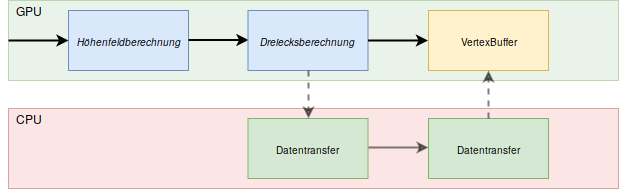
\includegraphics[scale=0.40]{img/pipeline.png}}
\label{fig:workflow}
\caption{Berechnungs- und Darstellungs-Workflow}
\end{figure}
W\"ahrend der Umsetzung des Projektes wurden zwei unterschiedliche Formen des Datenflusses implementiert. Abbildung \ref{fig:workflow} zeigt die zwei unterschiedlichen Vorgehensweisen. Zu Beginn des Projektes wurde nach Berechnung der Dreieckskoordinaten mit dem Kopieren der Kernelresultate zur\"uck zum Host ein unn\"otiger Umweg eingeschlagen. Im Laufe der Entwicklung hat sich herausgestellt, dass es wesentlich effizienter ist, die Kernelresultate im Speicher der GPU (im \textit{VertexBuffer}) zu belassen. In CUDA kann \"uber einen Pointer auf den Daten gearbeitet werden und OpenGL greift zum rendern der Daten auf den \textit{VertexBuffer} zu.

\subsection{Einf\"arbung der Wasseroberfl\"ache}
Die Einf\"arbung erfolgt anhand des Wertes der z-Koordinate. Ein 
\textit{Vertex-Shader} \"ubergibt einem \textit{Fragment-Shader} die Knotenpunkte der Dreiecke. Je nach z-Wert wird dann die Einf\"arbung mittels der OpenGL-Funktion \textit{mix()} realisiert. Diese Interpolationsfunktion erzeugt einen Gradienten von wei{\ss} bis blau und f\"arbt die Oberfl\"ache entsprechend ein.

\section{Auswertung}
In diesem Abschnitt erfolgt eine Bewertung einzelner Testszenarien. Zu diesem Zwecke wurden an markanten Stellen Zeitstempel gespeichert, um mit mikrosekundengenauen Zeitdifferenzen zu \"uberpr\"ufen wie sich die verschiedenen Konfigurationen auf die Laufzeit auswirken. Im Folgenden werden die farblich kodierten Konfigurationen kurz erkl\"art.


\begin{enumerate}
\item Rot: Alle Berechnungen erfolgen auf der CPU, die Grafikkarte wird nicht verwendet.
\item Blau: Alle Berechnungen erfolgen auf der GPU, ein R\"uckschreiben des Ergebnissen in den Host-Speicher ist nicht erforderlich.
\item Gr\"un: Alle Berechnungen erfolgen auf der GPU. Die Ergebnisse werden zur\"uck zum Host kopiert, der damit das \textit{Rendering} aktualisiert..
\end{enumerate}

Die folgenden Abbildungen zeigen auf der y-Achse die \"uber ca. 150.000 gemittelten Laufzeitwerte der jeweiligen auf der x-Achse abgetragenen Funktion in Mikrosekunden. Niedrigere Balken bedeuten daher bessere Performance. Der schwarze vertikale Strich innerhalb der Balken zeigt die Standardabweichung der jeweiligen Laufzeiten.

\begin{figure}[H]
\centerline{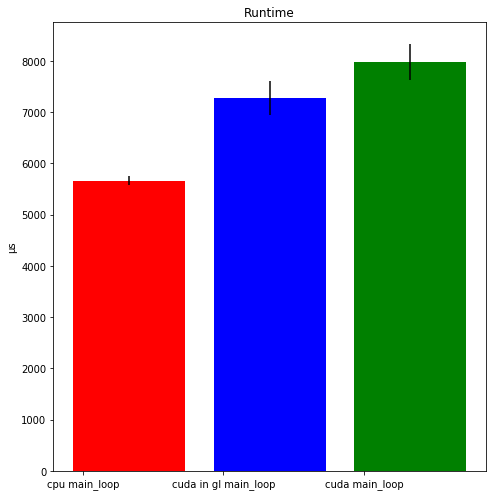
\includegraphics[scale=0.35]{img/main_loop_1threads.png}}
\label{fig:main_loop_1threads}
\caption{Main Loop - 1 Thread pro Block}
\end{figure}
Die y-Achse von Abbildung \ref{fig:main_loop_1threads} zeigt die Laufzeit f\"ur einen Rendering-Schritt. In diesem Testszenario wurde ein Thread pro Block gew\"ahlt. Da Bl\"ocke auf der Grafikkarte nicht parallel ausgef\"uhrt werden k\"onnen, findet hier eine sequentielle Abarbeitung statt. Wie am gr\"unen Balken zu erkennen, f\"uhrt der dadurch entstehende Overhead (wie etwa Kopiervorg\"ange, Taktung, ...) zu einer deutlich h\"oheren Laufzeit gegen\"uber der Ausf\"uhrung auf einem CPU-Kern.

\begin{figure}[H]
\centerline{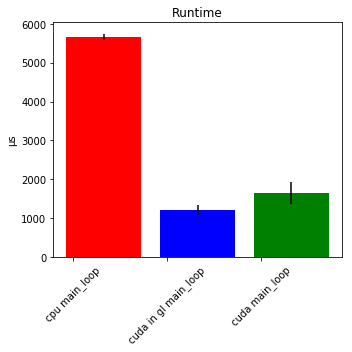
\includegraphics[scale=0.55]{img/main_loop_32threads.png}}
\label{fig:main_loop_32threads}
\caption{Main Loop - 1024 Thread pro Block}
\end{figure}
Abbildung \ref{fig:main_loop_32threads} zeigt die Berechnung mit der maximal m\"oglichen Anzahl an Threads pro Block. Dadurch reduzieren sich die Ausf\"uhrungszeiten drastisch, da hier jetzt eine echt-parallele Verarbeitung stattfindet. Die CPU rechnet immer noch mit einem Kern, die Laufzeit bleibt daher unver\"andert (siehe Abbildung \ref{fig:main_loop_1threads}). Durch Einsparungen von Kopiervorg\"angen zwischen Host und Device ist die "cuda in gl"-Implementierung performanter.

\begin{figure}[H]
\centerline{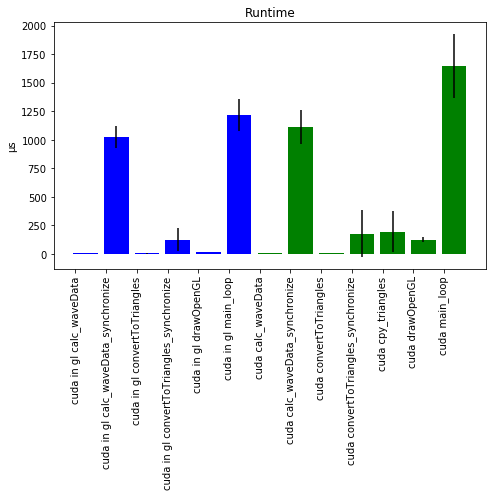
\includegraphics[scale=0.55]{img/cuda_vs_cudagl_32threads.png}}
\label{fig:cuda_vs_cudagl_32threads}
\caption{CUDA vs. CUDA-GL}
\end{figure}
Abbildung \ref{fig:cuda_vs_cudagl_32threads} stellt die zwei verschiedenen GPU-Implementierungen gegenuber. \textit{calc waveData} repr\"asentiert hier den Kernel zur Berechnung des H\"ohenfeldes. Der linke Balken zeigt das Triggern des Kernels, der folgende zeigt die eigentliche Laufzeit des Kernels. Analog dazu initiiert \textit{convertToTriangles}  widerrum den Kernel zur Berechnung der Dreiecke. \textit{drawOpenGL} st\"o{\ss}t das \textit{Rendering} an. Wird nicht nur auf der GPU gearbeitet (gr\"un), m\"ussen die errechneten Dreiecke mittels \textit{copyTriangles} erst zur\"uck zum Host und dann zum \textit{Rendering} kopiert werden. Diese Kopiervorg\"ange entfallen bei der reinen GPU-Implementierung, bei der \textit{drawOpenGL} deutlich schneller abl\"auft.

\section{Optimierung}\label{sec:optim}
Das Projekt  kann technisch noch an einigen Stellen verbessert werden. Beispielsweise wird im Status Quo die maximale Anzahl an Threads pro Block manuell eingetragen. Dies kann durch Abfragen dieser Konstante \"uber die \textit{deviceQuery} automatisiert werden. Ebenso k\"onnen, w\"ahrend CUDA-Kernel am rechnen sind, andere Operationen durchgef\"uhrt werden. Dies ist momentan ebenfalls nicht umgesetzt.\\
Eine mathematische Optimierung im Algorithmus kann ebenfalls vorgenommen werden: anstatt mit Funktion \ref{eq:ripples} das gesamte H\"ohenfeld mit allen Koordinaten zu berechnen, k\"onnte auch ein einzelner Strahl im Raum berechnet und dieser dann mittels geeigneter Transformationen \"uber die gesamte Fl\"ache projiziert werden.

\section{Fazit und Ausblick}
Bei diesem Projekt hat sich deutlich gezeigt, wie viel Performance-Zugewinn durch Parallelisierung von Programmcode und Einsetzen der Grafikkarte zu erreichen ist. Vor allem bei Anwendungen in der Computergrafik, wo Instruktionen auf ein gro{\ss}es Datenset angewandt werden, ist die Effizienz sp\"urbar. Voraussetzungen dafuer sind nat\"urlich die in Abschnitt \ref{sec:port} genannten Bedingungen f\"ur die Parallelisierung von Code.
Besondere Aufmerksamkeit ist der Konfiguration der Kernelparameter zu widmen. 
Zu beachten ist außerdem, dass nicht durch zu gro{\ss}z\"ugige Speicher-Allokationen der Zuwachs an Performance wieder zunichte gemacht wird.\\
Neben den im Abschnitt \ref{sec:optim} genannten Verbesserungen kann die Anwendung inhaltlich z.B. um die Darstellung multipler Ausbreitungszentren inkl. Wellen\"uberlagerung erweitert werden.

\section{Appendix}
Ein erster Gedanke bei Beginn des Projektes zur Umsetzung der Datenberechnung war, die gew\"unschte Anzahl an Koordinatenpaaren (x,y) zu generieren, um diese dann zur Berechnung der H\"ohenwerte innerhalb eines CUDA-Kernels zu nutzen. Dazu wurde ein Mechanismus implementiert, der sich an den bereits in \href{https://docs.scipy.org/doc/numpy/reference/generated/numpy.meshgrid.html}{Python (numpy)} oder \href{https://de.mathworks.com/help/matlab/ref/meshgrid.html}{Matlab} integrierten \textit{Meshgrid}-Funktionen orientiert und auf einen  von OrangeOwlSolutions implementierten \href{https://github.com/OrangeOwlSolutions/CUDA-Utilities/blob/master/Matlab_like.cu#L69}{Kernel} aufbaut.

\subsection{Meshgrid-Kernel}
Die entstandene Meshgrid-Funktion nimmt als Eingangsparameter Vektoren mit x- und y-Koordinaten und liefert dazu die entsprechenden x- und y-Koordinaten-Matrizen, die als Werte jeweils alle x- und y-Komponenten der gew\"unschten Koordinatenpaare enthalten:
\begin{lstlisting}[caption=Meshgrid-Generierung - Pseudo-Code, captionpos=b]
x = [1, 2]
y = [1, 2, 3]
step = 1
[X, Y] = gpuMeshgrid(x, y, step)

X = 5x3
	
	1	2	3
	1	2	3
	1	2	3
	1	2	3
	1	2	3
	
Y = 5x3
	
	1	1	1
	2	2	2
	3	3	3
	4	4	4
	5	5	5
\end{lstlisting}
Mit dem Parameter \textit{step} k\"onnen auch nicht-ganzzahlige Zwischenschritte erzeugt werden.\\Die Voraberzeugung der Koordinatenpaare ist jedoch nicht notwendig. Wie in Abschnitt \ref{sec:port} erl\"autert, werden die ben\"otigten Koordinatenpaare direkt w\"ahrend der Berechnung des H\"ohenfeldes generiert. Die angepasste Funktion und der erweiterte Kernel zur Meshgrid-Erzeugung wurde aber trotzdem als n\"utzliches Nebenprodukt des Projektes erachtet. 

\begin{thebibliography}{00}
\bibitem{onlPrimitives} 
Khronos - OpenGL: Primitives - Triangle Primitives,
\\\texttt{https://www.khronos.org/opengl/wiki/Primitive}
\end{thebibliography}

\end{document}